\documentclass[a4paper,12pt]{report}

\usepackage{graphicx}
\usepackage{amsmath}
\usepackage{fullpage}
\usepackage[parfill]{parskip}
\usepackage{amssymb}
\usepackage{alltt}
\usepackage{listings}

\newcommand{\degree}{\ensuremath{^\circ}}
\newcommand{\unit}[1]{\ensuremath{\, \mathrm{#1}}}

\begin{document}
\title{VirtualBox, Binary to Decimal Conversion and Networking Commands}
\author{Kimberley Manning}
\date{21 September 2012}
\newpage

\section*{COMP30040 - Assignment 2}

\subsubsection*{Wireshark (Packet Analysis) and IP Address Configuration}

\textbf{Question 1}

The following commands can be used to examine the IP configuration:

\begin{itemize}
\item \verb=ifconfig:= configure or display statistics on a network interface, such as the IP address, netmask and MAC address
\item \verb=route:= show the IP routing table (with \verb=-n=: show numerical addresses instead of host names), which is used to figure out a path to the destination network of a packet - or to a gateway in the network, which will figure it out
\end{itemize}

\begin{alltt}
[kimberley@promethei ~]$ ifconfig wlan0
wlan0: flags=4163<UP,BROADCAST,RUNNING,MULTICAST>  mtu 1500
inet 137.43.68.127  netmask 255.255.255.0  broadcast 137.43.68.255
inet6 fe80::2b9:a5ff:fed2:cfbb  prefixlen 64  scopeid 0x20<link>
ether e0:b9:a5:d2:cf:bb  txqueuelen 1000  (Ethernet)
RX packets 11769  bytes 5844746 (5.5 MiB)
RX errors 0  dropped 0  overruns 0  frame 0
TX packets 8188  bytes 1260157 (1.2 MiB)
TX errors 0  dropped 0 overruns 0  carrier 0  collisions 0

[kimberley@promethei ~]$ route -n
Kernel IP routing table
Destination     Gateway         Genmask         Flags Metric Ref    Use Iface
0.0.0.0         137.43.68.1     0.0.0.0         UG    0      0        0 wlan0
137.43.68.0     0.0.0.0         255.255.255.0   U     0      0        0 wlan0

\end{alltt}

From this we can tell the following:

\begin{itemize}
\item IP address: \verb=137.43.68.127=
\item netmask: \verb=255.255.255.0=
\item gateway: \verb=137.43.68.1=
\item MAC address: \verb=e0:b9:a5:d2:cf:bb=
\end{itemize}

Interestingly enough these two commands - and a related one, \verb=arp=, which relates MAC addresses to IP addresses - state that they are obsolete in their respective man pages. Alright. Let's try the suggested replacement, \verb=ip=:

\begin{alltt}

[kimberley@promethei ~]$ ip
Usage: ip [ OPTIONS ] OBJECT { COMMAND | help }
       ip [ -force ] -batch filename
where  OBJECT := { link | addr | addrlabel | route | rule | neigh | ntable |
                   tunnel | tuntap | maddr | mroute | mrule | monitor | xfrm |
                   netns | l2tp }
       OPTIONS := { -V[ersion] | -s[tatistics] | -d[etails] | -r[esolve] |
                    -f[amily] { inet | inet6 | ipx | dnet | link } |
                    -l[oops] { maximum-addr-flush-attempts } |
                    -o[neline] | -t[imestamp] | -b[atch] [filename] |
                    -rc[vbuf] [size]}
                                                                                        \end{alltt}

With \verb=-s=, it will display different statistics depending on the objects specified. The relevant ones are \verb=addr=, which gives similar information to \verb=ifconfig=, and \verb=route=, which unsurprisingly gives similar information to \verb=route=.

\begin{alltt}
[kimberley@promethei ~]$ ip -s addr
1: lo: <LOOPBACK,UP,LOWER_UP> mtu 16436 qdisc noqueue state UNKNOWN 
    link/loopback 00:00:00:00:00:00 brd 00:00:00:00:00:00
    inet 127.0.0.1/8 scope host lo
    inet6 ::1/128 scope host 
       valid_lft forever preferred_lft forever
2: wlan0: <BROADCAST,MULTICAST,UP,LOWER_UP> mtu 1500 qdisc mq state UP qlen 1000
    link/ether e0:b9:a5:d2:cf:bb brd ff:ff:ff:ff:ff:ff
    inet 137.43.68.127/24 brd 137.43.68.255 scope global wlan0
    inet6 fe80::e2b9:a5ff:fed2:cfbb/64 scope link 
       valid_lft forever preferred_lft forever

\end{alltt}

Note: instead of specifying the netmask in dotted decimal notation, it is given in something called CIDR notation. The number after the slash in \verb=137.43.68.127/24= is the number of bits allocated to the network prefix (the part of the IP address which specifies the network), with the remaining bits identifying the specific host on the network. \verb=/24= is equivalent to the subnet mask \verb=255.255.255.0=.

\begin{alltt}
[kimberley@promethei ~]$ ip -s route
default via 137.43.68.1 dev wlan0  proto static 
137.43.68.0/24 dev wlan0  proto kernel  scope link  src 137.43.68.127 
\end{alltt}

Once again we can see that the default gateway is \verb=137.43.68.1=.

\newpage

\textbf{Question 2}

Before reconfiguration, my Ubuntu VM's IP address is \verb=10.0.2.15= (assignment 1).

After editing \verb=/etc/network/interfaces=:

\begin{alltt}
root@tempe:/home/kimberley# cat /etc/network/interfaces
auto lo
iface lo inet loopback

auto eth0
iface eth0 inet static
address 10.0.2.14
netmask 255.255.255.0
gateway 10.0.2.2
dns-nameservers 137.43.116.19
\end{alltt}

Switch to static network configuration:

\begin{alltt}
root@tempe:/home/kimberley# service network-manager stop
network-manager stop/waiting
root@tempe:/home/kimberley# ifdown eth0
root@tempe:/home/kimberley# ifup eth0
\end{alltt}

Test connectivity:

\begin{alltt}
root@tempe:/home/kimberley# ping google.com -q -c5
PING google.com (74.125.24.101) 56(84) bytes of data.

--- google.com ping statistics ---
5 packets transmitted, 0 received, 100% packet loss, time 4033ms

root@tempe:/home/kimberley# telnet google.com 80
Trying 74.125.24.139...
Connected to google.com.
Escape character is '^]'.
^]

telnet> quit
Connection closed.
root@tempe:/home/kimberley# ping 137.43.68.127 -q -c5
PING 137.43.68.127 (137.43.68.127) 56(84) bytes of data.

--- 137.43.68.127 ping statistics ---
5 packets transmitted, 5 received, 0% packet loss, time 3999ms
rtt min/avg/max/mdev = 0.178/0.480/1.282/0.407 ms
\end{alltt}

I have no idea why it won't let me ping google - but I can connect to my host machine as well as telnet to google.com, so I clearly still have a connection to the outside world and DNS is working.

\textbf{Question 3}

Address Resolution Protocol (ARP) is used to map MAC addresses (of physical hardware) to IP addresses.

Generate ARP packages by pinging another host on the network (machine with IP address \verb=137.43.68.123=). First confirm that there is no ARP entry for that IP address, meaning an ARP request will have to be sent.

\begin{alltt}
[kimberley@promethei ~]$ sudo arp -d 137.43.68.123
No ARP entry for 137.43.68.123
\end{alltt}

Start capturing ARP packages on wlan0 using Wireshark:

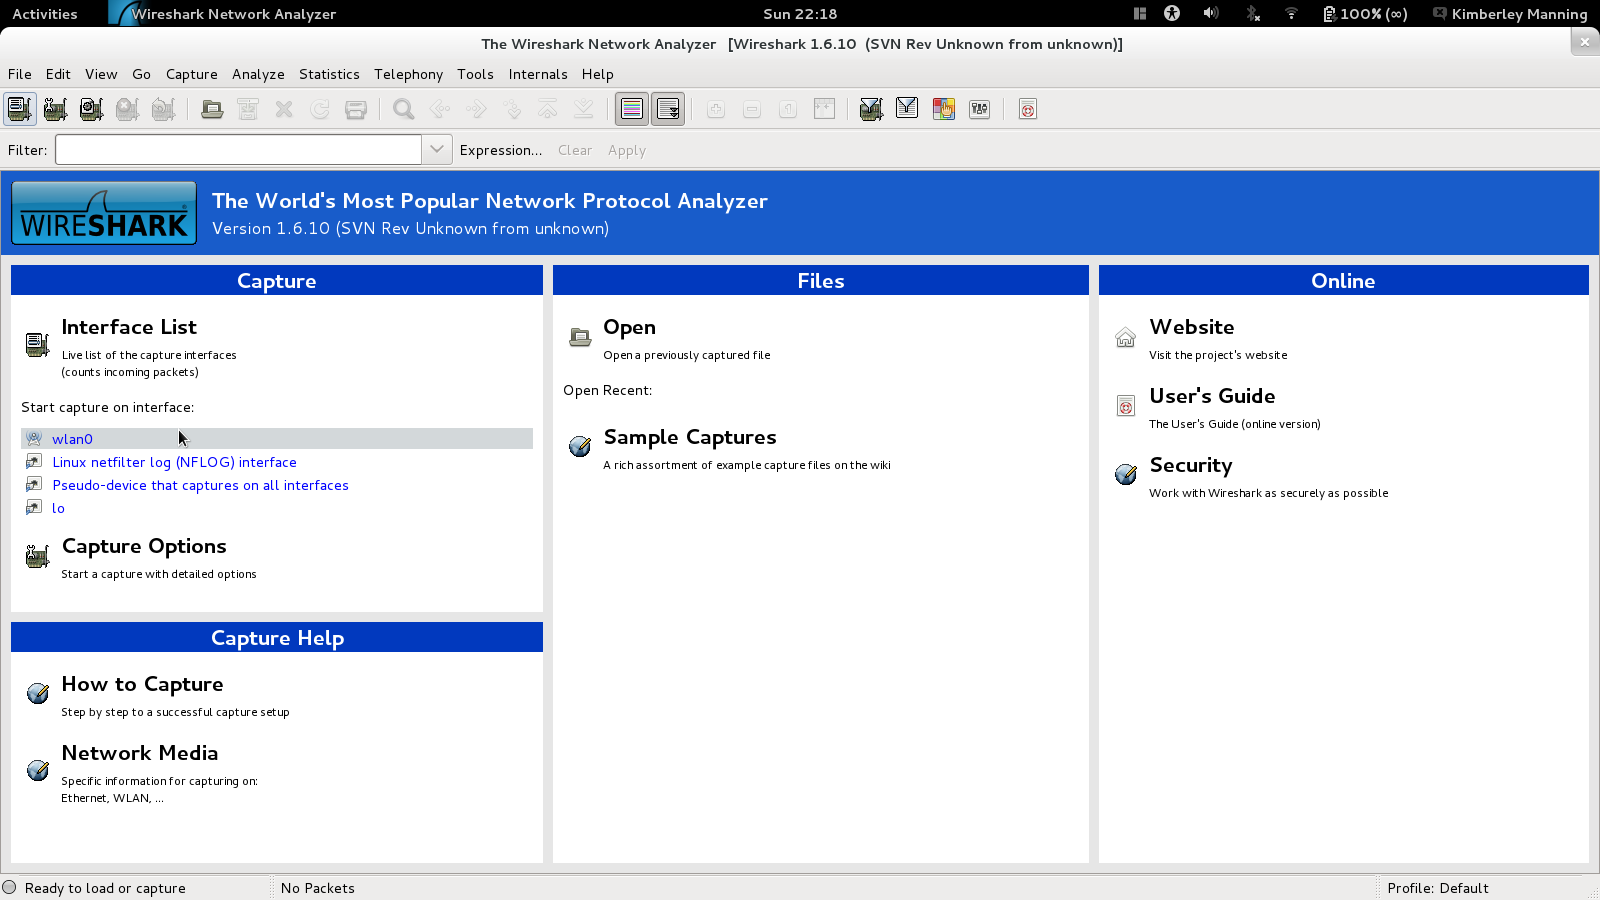
\includegraphics[width=\textwidth]{start.png}

Now begin pinging the destination IP:

\begin{alltt}
[kimberley@promethei ~]$ ping 137.43.68.123 -q -c5
PING 137.43.68.123 (137.43.68.123) 56(84) bytes of data.

--- 137.43.68.123 ping statistics ---
5 packets transmitted, 4 received, 20% packet loss, time 4004ms
rtt min/avg/max/mdev = 2.443/12.598/41.103/16.462 ms
\end{alltt}

\newpage

In Wireshark, filter out all but ARP packages:

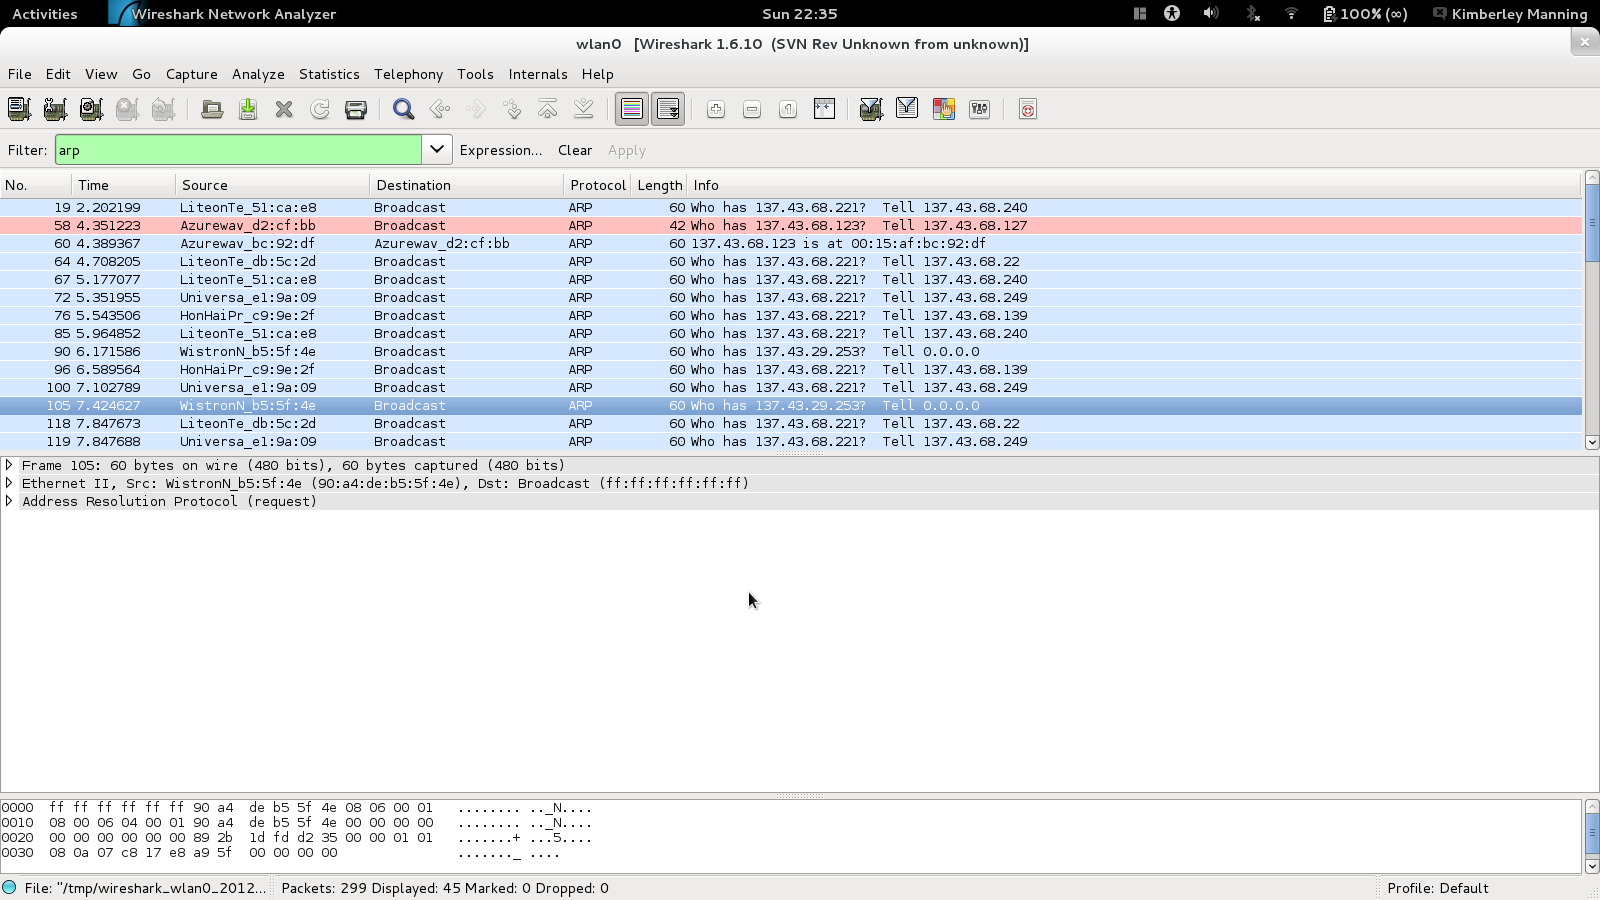
\includegraphics[width=\textwidth]{found.png}

You can also see the 5 pings and responses between the source machine (\verb=137.43.68.127=) and the destination machine (\verb=137.43.68.123=). Note that the destination is on the same network as the source, because it makes no sense to have ARP table entries for machines on a different network.

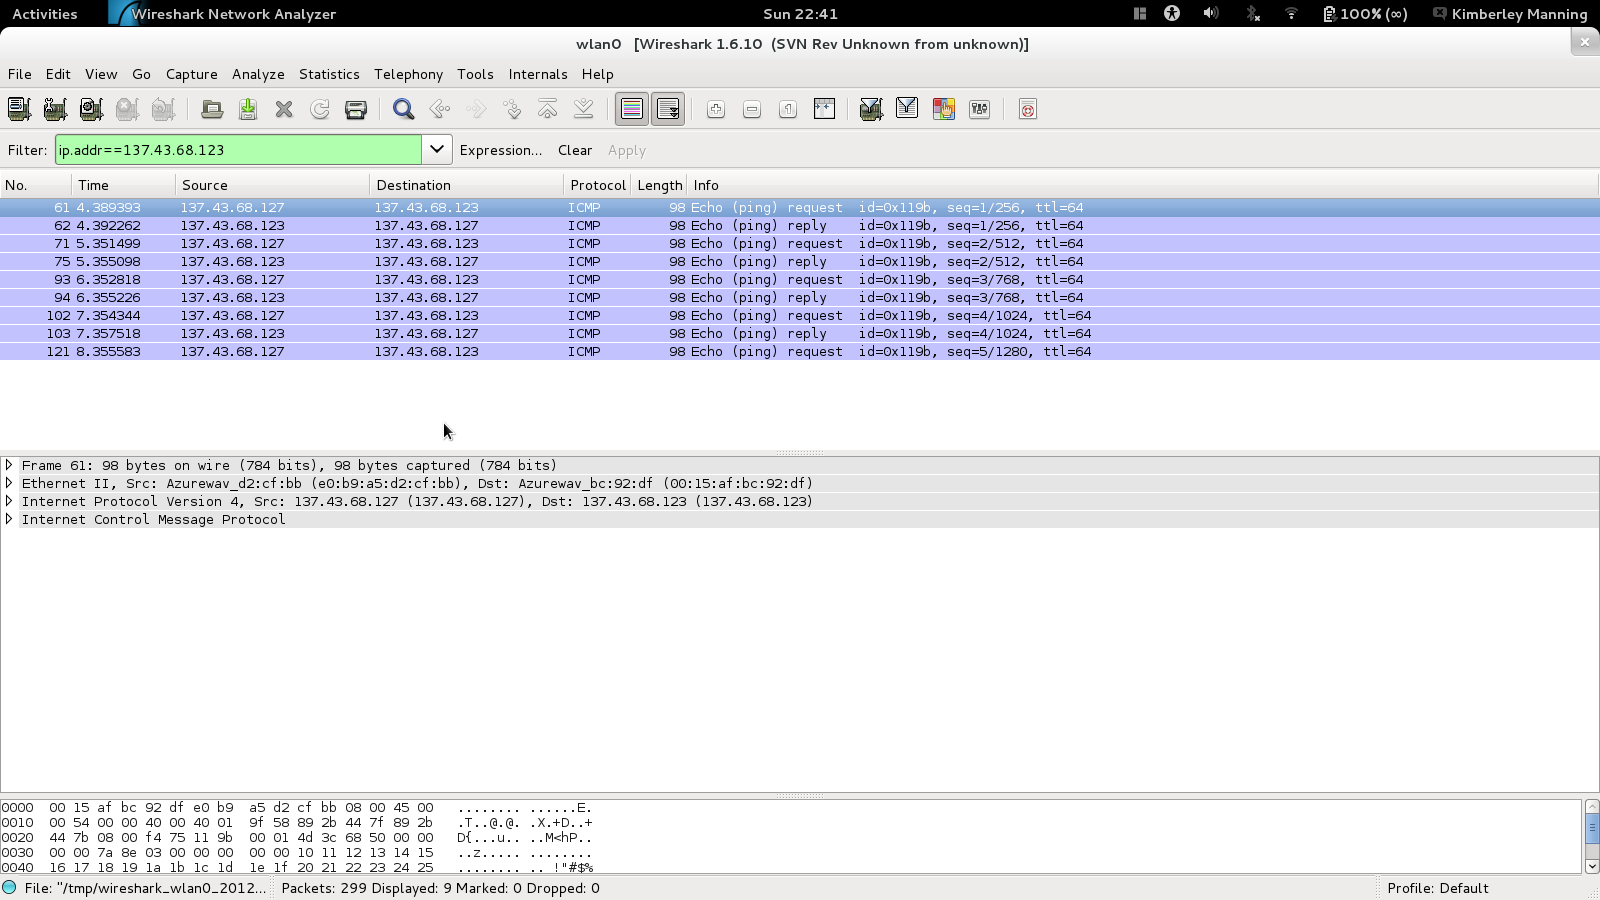
\includegraphics[width=\textwidth]{search.png}



\end{document}
